\section{Discussion}

There remains some interesting aspects that can be potentially helpful for better scene understanding.
First, it maybe be worth some effort of a better choice of hyper-parameters, such as grid size, number of quantized directions, video clip length, length training video, maximal sampling iterations.
Grid size is related to the frame size. It is may not be necessary to have the same grid size for videos with different resolutions, since smaller grid size results in a larger vocabulary and a longer training time.
For videos with only horizontal and vertical motions, the optical flow quantization can be sparser. 
The video clip length may also need to adjust depending on different scenarios: ideally, we expect a video clip to cover a complete lifetime of single motion; shorter clip may break a topic into different parts while a longer video clip may generate a topic with mixed motions. 
Also, we have consider the traffic density of the scene to choose the size of the training data.
A scene with little traffic needs a longer training video than a crowded one.
However, even though the topic model is trained on a longer video, some rare motions may still be missing.


In addition, adding constraints among visual words might be necessary for some busy interactions. 
A ``topic'' is interpreted as a cluster containing ``words'' that always appear together, where the ``words'' are treated independently.
For an intersection with bi-directional movements all the time, the movement on both direction is naturally clustered as a single ``topic''. 
However, under the context of a video, the ``visual words'' are spatially and temporarily connected. 
If a ``visual topic'' is defined with only a single motion, the ``visual words'' one the opposite direction should be mutually exclusive.
\ref{fig:entry-exit-fail-1} and \ref{fig:entry-exit-fail-2} show two failure cases. 
One or more topics contain mixed motions, since those motion always happen simultaneously in the training data.
\begin{figure}
    \centering
        \begin{subfigure}{0.32\linewidth}
            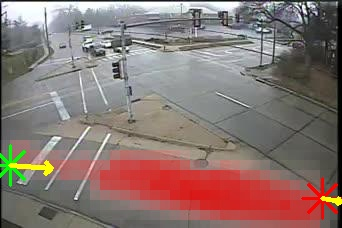
\includegraphics[width=\linewidth]{./img/scene_learning/res/243653/243653_h264_0-0.jpg}
        \end{subfigure}
        \begin{subfigure}{0.32\linewidth}
            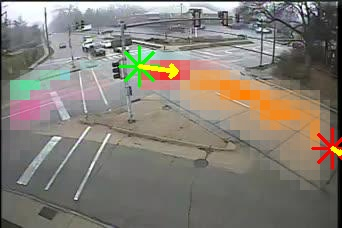
\includegraphics[width=\linewidth]{./img/scene_learning/res/243653/243653_h264_0-1.jpg}
        \end{subfigure}
        \begin{subfigure}{0.32\linewidth}
            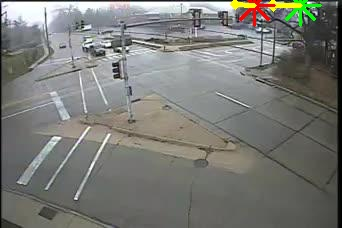
\includegraphics[width=\linewidth]{./img/scene_learning/res/243653/243653_h264_0-2.jpg}
        \end{subfigure}
        \caption{Failure case with simultaneous opposite directions. Entry (green) and exit (red) locations with direction (yellow arrows).}
        \label{fig:entry-exit-fail-1}
\end{figure}
\begin{figure}
    \centering
        \begin{subfigure}{0.32\linewidth}
            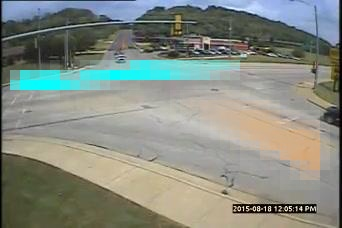
\includegraphics[width=\linewidth]{./img/scene_learning/res/251950/251950-0.jpg}
        \end{subfigure}
        \begin{subfigure}{0.32\linewidth}
            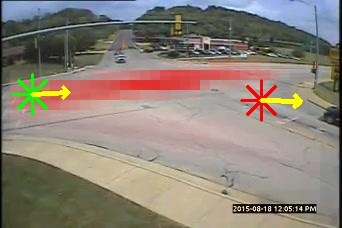
\includegraphics[width=\linewidth]{./img/scene_learning/res/251950/251950-1.jpg}
        \end{subfigure}

        \begin{subfigure}{0.32\linewidth}
            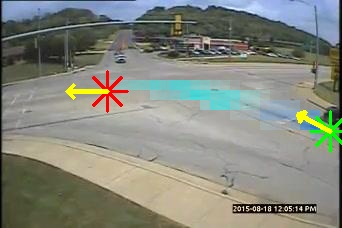
\includegraphics[width=\linewidth]{./img/scene_learning/res/251950/251950-2.jpg}
        \end{subfigure}
        \begin{subfigure}{0.32\linewidth}
            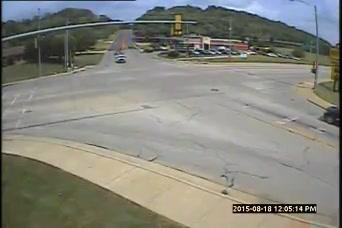
\includegraphics[width=\linewidth]{./img/scene_learning/res/251950/251950-3.jpg}
        \end{subfigure}
        \caption{Failure case with simultaneous opposite directions. Entry (green) and exit (red) with direction (yellow arrows) at a crowded intersection.}
        \label{fig:entry-exit-fail-2}
\end{figure}


However, if the training video is carefully chosen, this problem may be avoided.
\ref{fig:entry-exit-night-1} and \ref{fig:entry-exit-night-2} are visualization of two models trained on a night video with sparse traffic. 
\ref{fig:entry-exit-night-1} is trained on a 5-minutes video, and \ref{fig:entry-exit-night-2} is trained on a 30-minutes video.
Topics in \ref{fig:entry-exit-night-2} have a better interpretation of the scene because the training video has sparse traffic at night. 
Since the video contain little traffic, there is less likely to have simultaneous movement in the opposite direction.
A longer video has much more sufficient data for training.
\begin{figure}
    \centering
        \begin{subfigure}{0.32\linewidth}
            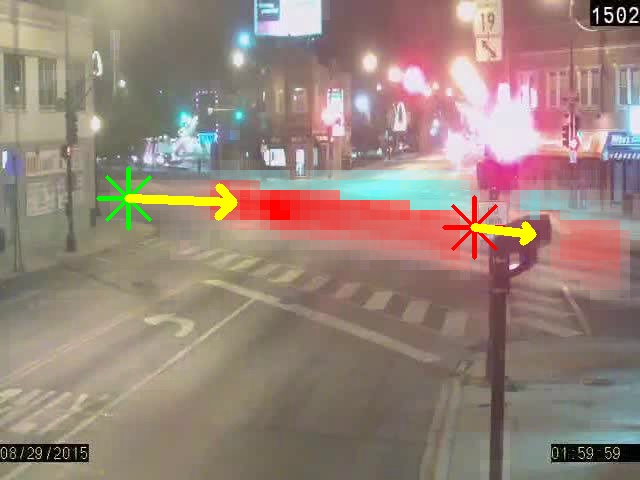
\includegraphics[width=\linewidth]{./img/scene_learning/res/elstonIrvingPark-short/20150829_020000DST_elstonIrvingPark-0.jpg}
        \end{subfigure}
        \begin{subfigure}{0.32\linewidth}
            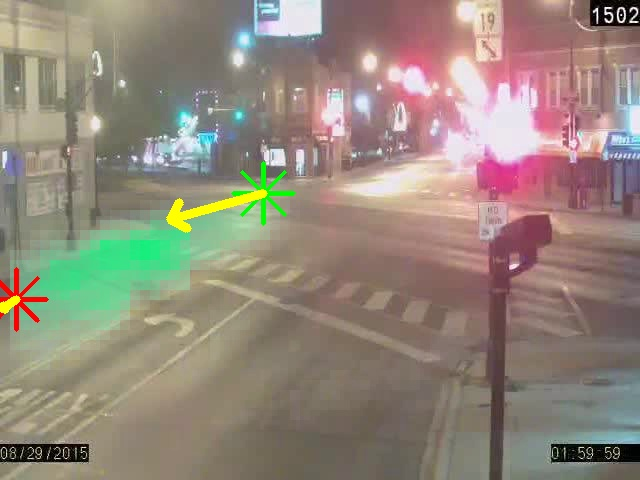
\includegraphics[width=\linewidth]{./img/scene_learning/res/elstonIrvingPark-short/20150829_020000DST_elstonIrvingPark-1.jpg}
        \end{subfigure}
        \begin{subfigure}{0.32\linewidth}
            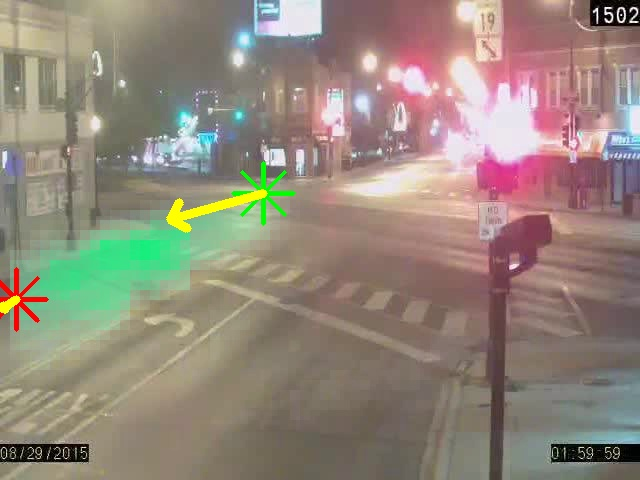
\includegraphics[width=\linewidth]{./img/scene_learning/res/elstonIrvingPark-short/20150829_020000DST_elstonIrvingPark-1.jpg}
        \end{subfigure}

        \begin{subfigure}{0.32\linewidth}
            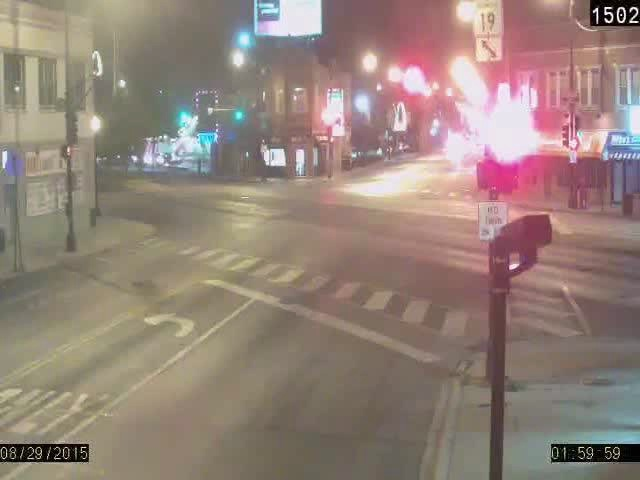
\includegraphics[width=\linewidth]{./img/scene_learning/res/elstonIrvingPark-short/20150829_020000DST_elstonIrvingPark-3.jpg}
        \end{subfigure}
        \begin{subfigure}{0.32\linewidth}
            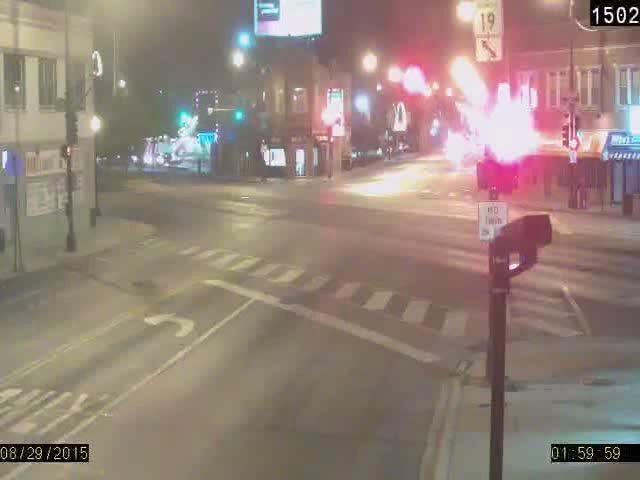
\includegraphics[width=\linewidth]{./img/scene_learning/res/elstonIrvingPark-short/20150829_020000DST_elstonIrvingPark-4.jpg}
        \end{subfigure}
        \caption{Model training on sparse night video about 5 minutes. Entry (green) and exit (red) locations with direction (yellow arrows).}
        \label{fig:entry-exit-night-1}
\end{figure}
\begin{figure}
    \centering
        \begin{subfigure}{0.32\linewidth}
            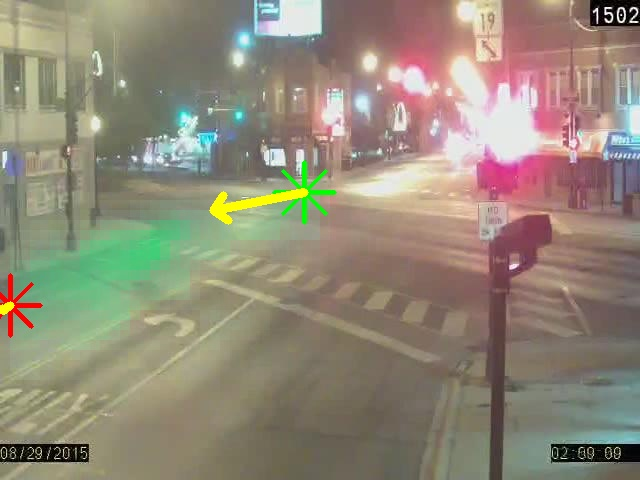
\includegraphics[width=\linewidth]{./img/scene_learning/res/elstonIrvingPark/20150829_020000DST_elstonIrvingPark-0.jpg}
        \end{subfigure}
        \begin{subfigure}{0.32\linewidth}
            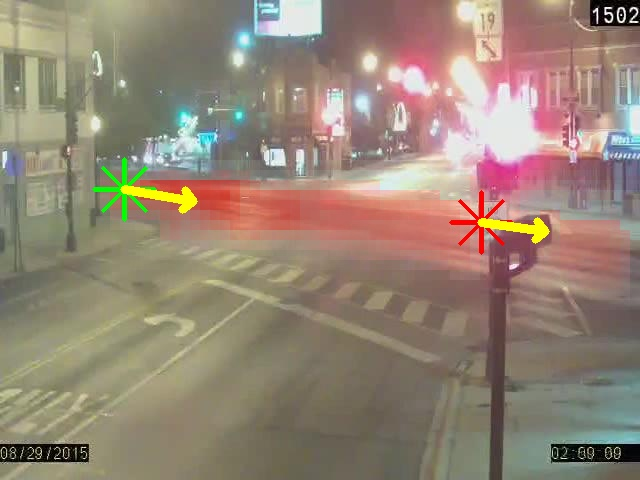
\includegraphics[width=\linewidth]{./img/scene_learning/res/elstonIrvingPark/20150829_020000DST_elstonIrvingPark-1.jpg}
        \end{subfigure}

        \begin{subfigure}{0.32\linewidth}
            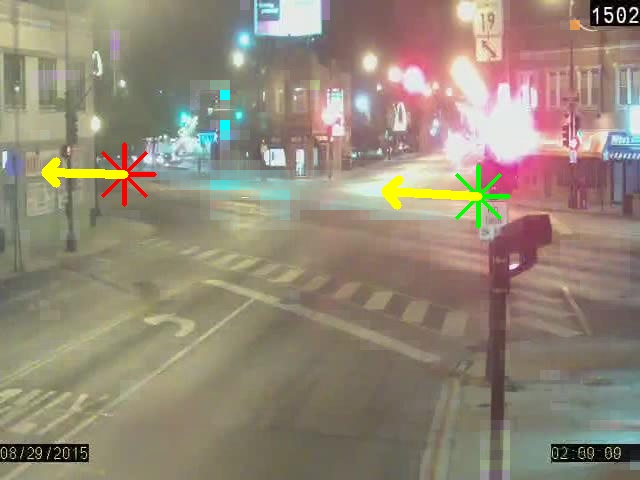
\includegraphics[width=\linewidth]{./img/scene_learning/res/elstonIrvingPark/20150829_020000DST_elstonIrvingPark-2.jpg}
        \end{subfigure}
        \begin{subfigure}{0.32\linewidth}
            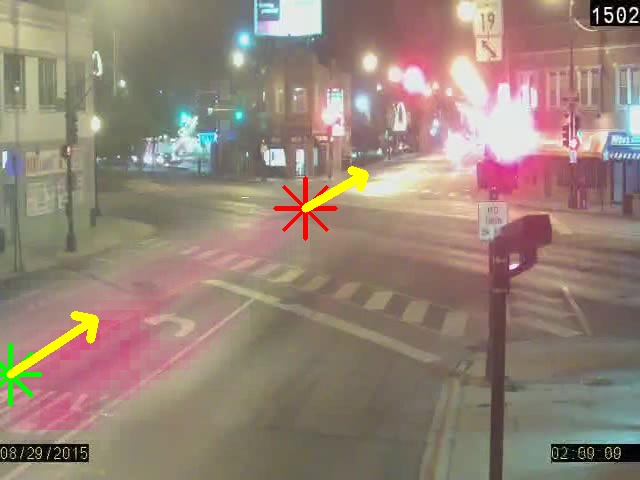
\includegraphics[width=\linewidth]{./img/scene_learning/res/elstonIrvingPark/20150829_020000DST_elstonIrvingPark-3.jpg}
        \end{subfigure}
        \caption{Model training on sparse night video about 30 minutes. Entry (green) and exit (red) locations with direction (yellow arrows).}
        \label{fig:entry-exit-night-2}
\end{figure}


However, it does not always work for tuning training videos. 
If a busy intersection always have the opposite movement at the same time, the learned topics tend to contain mixed movement.
We considered introducing such exclusion into \gls{hdp} via Hierarchical \gls{ddcrp} \cite{blei2011distance}.
Due to the limited time, we do not completely finish this part.